% Figure M2, generated by experiments/m2_monosemanticity.py.
\begin{figure}[t]
  \centering
  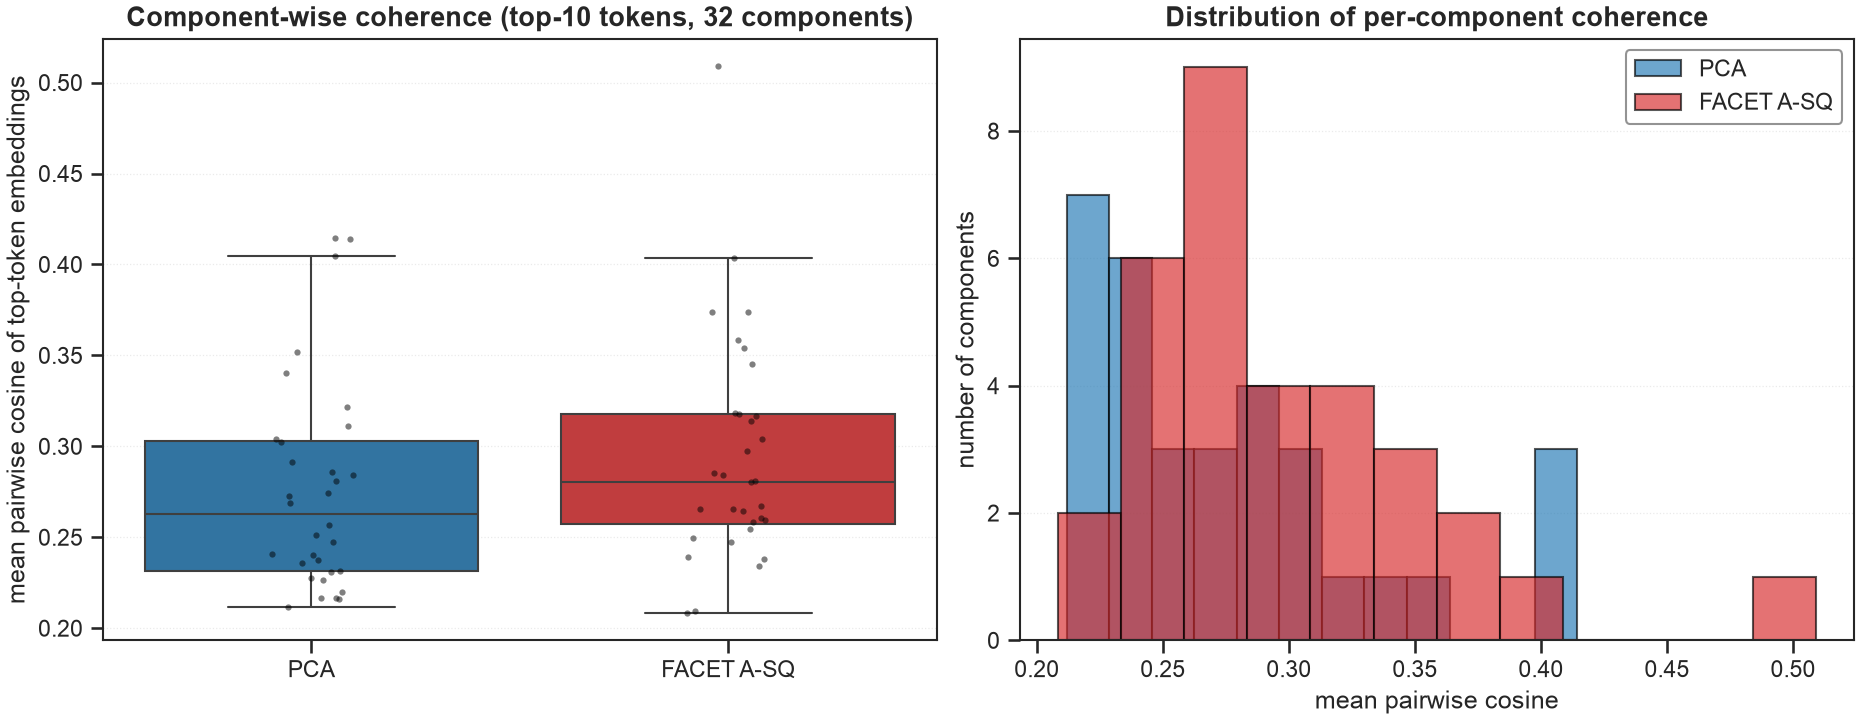
\includegraphics[width=\linewidth]{../shared/figures/generated/m2_monosemanticity.png}
  \caption{\textbf{M2, top-token coherence (GPT-2 block 4 \texttt{attn\_out}).} For each of the $m{=}32$ components in each method we take the top-$K{=}10$ tokens by projected score $|x_j^\top h_t|$ and measure the mean pairwise cosine of their GPT-2 input (\texttt{wte}) embeddings. Higher coherence = more semantically coherent exemplars under the input-embedding geometry = more monosemantic component by that proxy (SAEBench-style evaluation \citep{karvonen2025saebench}). \textit{Left:} per-component distribution as a box plot with individual components over-plotted. \textit{Right:} histograms of the same distribution. FACET components have higher median coherence (0.28 vs PCA 0.26) and a longer upper tail (max 0.51 vs 0.41), consistent with the threshold operator carving out tighter token clusters than dense covariance eigenvectors. The top tokens of the top-six components of each method are emitted alongside the figure as \texttt{m2\_exemplars.json}.}
  \label{fig:m2-monosemanticity}
\end{figure}
